\documentclass[12pt,a4paper]{article}
%\usepackage{ctex}
\usepackage{amsmath,amscd,amsbsy,amssymb,latexsym,url,bm,amsthm}
\usepackage{epsfig,graphicx,subfigure}
\usepackage{enumitem,balance}
\usepackage{wrapfig}
\usepackage{mathrsfs,euscript}
\usepackage[x11names,svgnames,dvipsnames]{xcolor}
\usepackage{hyperref}
\usepackage[vlined,ruled,commentsnumbered,linesnumbered]{algorithm2e}
\usepackage{listings}
\usepackage{multicol}
%\usepackage{fontspec}

\renewcommand{\listalgorithmcfname}{List of Algorithms}
\renewcommand{\algorithmcfname}{Alg.}
\newtheorem{theorem}{Theorem}
\newtheorem{lemma}[theorem]{Lemma}
\newtheorem{proposition}[theorem]{Proposition}
\newtheorem{corollary}[theorem]{Corollary}
\newtheorem{exercise}{Exercise}
\newtheorem*{solution}{Solution}
\newtheorem{definition}{Definition}
\theoremstyle{definition}


%\numberwithin{equation}{section}
%\numberwithin{figure}{section}

\renewcommand{\thefootnote}{\fnsymbol{footnote}}

\newcommand{\postscript}[2]
 {\setlength{\epsfxsize}{#2\hsize}
  \centerline{\epsfbox{#1}}}

\renewcommand{\baselinestretch}{1.0}

\setlength{\oddsidemargin}{-0.365in}
\setlength{\evensidemargin}{-0.365in}
\setlength{\topmargin}{-0.3in}
\setlength{\headheight}{0in}
\setlength{\headsep}{0in}
\setlength{\textheight}{10.1in}
\setlength{\textwidth}{7in}
\makeatletter \renewenvironment{proof}[1][Proof] {\par\pushQED{\qed}\normalfont\topsep6\p@\@plus6\p@\relax\trivlist\item[\hskip\labelsep\bfseries#1\@addpunct{.}]\ignorespaces}{\popQED\endtrivlist\@endpefalse} \makeatother
\makeatletter
\renewenvironment{solution}[1][Solution] {\par\pushQED{\qed}\normalfont\topsep6\p@\@plus6\p@\relax\trivlist\item[\hskip\labelsep\bfseries#1\@addpunct{.}]\ignorespaces}{\popQED\endtrivlist\@endpefalse} \makeatother


\definecolor{codegreen}{rgb}{0.44,0.68,0.28}
\definecolor{codegray}{rgb}{0.5,0.5,0.5}
\definecolor{codepurple}{rgb}{0.58,0,0.82}
\definecolor{backcolour}{rgb}{0.96,0.96,0.96}

\lstset{
language=C++,
frame=shadowbox,
keywordstyle = \color{blue}\bfseries,
commentstyle=\color{codegreen},
tabsize = 4,
backgroundcolor=\color{backcolour},
numbers=left,
numbersep=5pt,
breaklines=true,
emph = {int,float,double,char},emphstyle=\color{orange},
emph ={[2]const, typedef},emphstyle = {[2]\color{red}} }



\begin{document}
\noindent

%========================================================================
\noindent\framebox[\linewidth]{\shortstack[c]{
\Large{\textbf{Lab08-Graphs}}\vspace{1mm}\\
VE281 - Data Structures and Algorithms, Xiaofeng Gao, TA: Li Ma, Autumn 2019}}
%CS26019 - Algorithm Design and Analysis, Xiaofeng Gao, Autumn 2019}}
\begin{center}
\footnotesize{\color{red}$*$ Please upload your assignment to website. Contact webmaster for any questions.}

\footnotesize{\color{blue}$*$ Name: Sun Yiwen  \quad Student ID: 517370910213 \quad Email: sunyw99@sjtu.edu.cn}
\end{center}


\begin{enumerate}

\item \textbf{DAG.} Suppose that you are given a directed acyclic graph $G=(V,E)$ with real-valued edge weights and two distinct nodes $s$ and $d$. Describe an algorithm for finding a longest weighted simple path from $s$ to $d$. For example, for the graph shown in Figure 1, the longest path from node $A$ to node $C$ should be $A \rightarrow B \rightarrow F \rightarrow C$. If there is no path exists between the two nodes, your algorithm just tells so. What is the efficiency of your algorithm? (Hint: consider topological sorting on the DAG.)

\begin{solution}
\ \\
\begin{minipage}[t]{0.47\textwidth}
\begin{algorithm}[H]
	\caption{longestPath(G,s,d)}
	\KwIn{graph $G$ = ($V$, $E$), directed; vertex $s$ $\in$ $V$; vertex $d$ $\in$ $V$}
	\KwOut{a stack $S$ of nodes that demonstrates the longest weighted simple path from node $s$ to node $d$, with node $s$ on the top and $d$ in the bottom}
	\For {each $u\in V$}
	{
		$dist[u]=-\infty$;
	}
	$dist[s]=0$;\\
	topologicalSort($G$);\\
	\For{each $u\in V$ in topological order}
	{
		\For{each $v\in Adj[u]$}
		{
			\If {$dist[v]<dist[u]+w(u,v)$}
			{
				$dist[v]\leftarrow dist[u]+w(u,v)$;
			} 
		}
	}
	Create $G^R=(V',E')$ as the reverse graph of $G$.\\
	vertex $temp\leftarrow d$;\\
	S.push($d$);\\
	\While {$temp!=s$}
	{
		\For {each $v\in Adj[temp]$}
		{
			\If{$dist[temp]==dist[v]+w(temp,v)$}
			{
				$temp\leftarrow v$;\\
				S.push($v$);
			}
		}
	}
\end{algorithm}
\end{minipage}
\hspace{2mm}
\begin{minipage}[t]{0.47\textwidth}
\begin{algorithm}[H]
	\caption{topologicalSort($G$)}
	\KwIn{graph $G$ = ($V$, $E$), directed}
	\KwOut{a stack $S$ of nodes}
	Mark all the nodes as not visited;\\
	\For{each $u\in V$}
	{
		\If{$u$ is not visited}
		{
			topologicalSort$\_$help($u$,$S$);
		}
	}
\end{algorithm}
\begin{algorithm}[H]
	\caption{topologicalSort$\_$help($u$,$S$)}
	\KwIn{vertex $u$,stack $S$}
	Set $u$ as visited;\\
	\For{each $v\in Adj[u]$}
	{
		\If{$v$ is not visited}
		{
			topologicalSort$\_$help($v$,$S$);
		}
		S.push($v$);
	}
\end{algorithm}
The time complexity of my algorithm is $O(|V|+|E|)$.
\end{minipage}
\end{solution}

\begin{figure}[htbp]
% \begin{minipage}[t]{0.5\linewidth}
% \centering
% 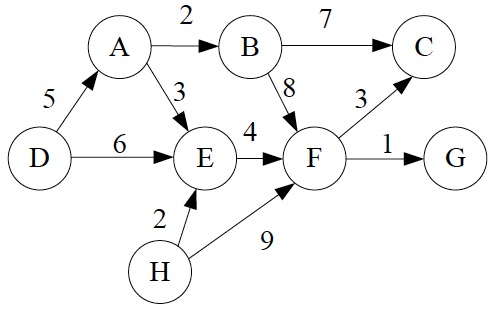
\includegraphics[scale=0.35]{Lab08-figure1.jpg}
% \caption{A weighted undirected graph.}
% \end{minipage}%
% \begin{minipage}[t]{0.5\linewidth}
\centering
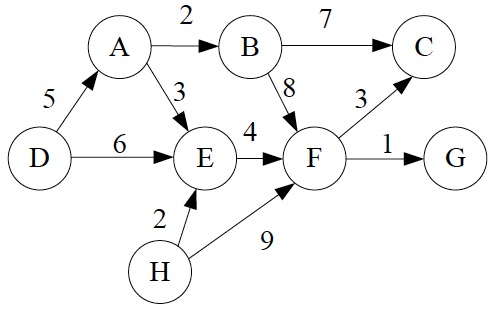
\includegraphics[scale=0.35]{Lab08-figure1.jpg}
\caption{A weighted directed graph.}
% \end{minipage}
\end{figure}

\item \textbf{ShortestPath.} Suppose that you are given a directed graph $G=(V,E)$ on which each edge $(u,v) \in E$ has an associated value $r(u,v)$, which is a real number in the range $0 \leq r(u,v) \leq 1$ that represents the reliability of a communication channel from vertex $u$ to vertex $v$. We interpret $r(u,v)$ as the probability that the channel from $u$ to $v$ will not fail, and we assume that these probabilities are independent. Give an efficient algorithm to find the most reliable path between two given vertices.

\begin{solution}
\ \\
\begin{minipage}[t]{0.9\textwidth}
\begin{algorithm}[H]
	\caption{shortestPath(G,s,d)}
	\KwIn{graph $G$ = ($V$, $E$), directed; vertex $s$ $\in$ $V$; vertex $d$ $\in$ $V$}
	\KwOut{a stack $S$ of vertexes that demonstrates the most reliable path from vertex $s$ to vertex $d$, with $s$ on the top and $d$ in the bottom}
	\For{each $u\in V$}
	{
		$dist[u]=\infty$;
	}
	$dist[s]=1$;\\
	\For{each $u\in V$}
	{
		INSERT($Q,u$);
	}
	\While{$Q$ is not empty}
	{
		$u\leftarrow$EXTRACT-MIN($Q$);\\
		$S\leftarrow S\cup\{u\}$;\\
		\For{each $v\in Adj[u]$}
		{
			\If{$dist[v]>dist[u]*r(u,v)$}
			{
				$dist[v]\leftarrow dist[u]*r(u,v)$;
				DECREASE-KEY($Q,v$);
			}
		}
	}
	Create $G^R=(V',E')$ as the reverse graph of $G$.\\
	vertex $temp\leftarrow d$;\\
	S.push($d$);\\
	\While {$temp!=s$}
	{
		\For {each $v\in Adj[temp]$}
		{
			\If{$dist[temp]==dist[v]*r(temp,v)$}
			{
				$temp\leftarrow v$;\\
				S.push($v$);
			}
		}
	}
\end{algorithm}
\end{minipage}		
\end{solution}

\item \textbf{GraphSearch.} Let $G=(V,E)$ be a connected, undirected graph. Give an $O(|V|+|E|)$-time algorithm to compute a path in $G$ that traverses each edge in $E$ \textbf{exactly once in each direction}. For example, for the graph shown in Figure 2, one path satisfying the requirement is
$$A \rightarrow B \rightarrow C \rightarrow D \rightarrow C \rightarrow A \rightarrow C \rightarrow B \rightarrow A$$
Note that in the above path, each edge is visited exactly once in each direction.

\begin{figure}[h]
 \centering
 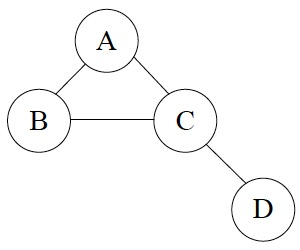
\includegraphics[scale=0.35]{Lab08-figure2.jpg}
 \caption{A undirected graph.}
\end{figure}

\begin{solution}
\ \\
\begin{minipage}[t]{0.47\textwidth}
\begin{algorithm}[H]
	\caption{graphSearch(G)}
	\KwIn{graph $G$ = ($V$, $E$)}
	\KwOut{a stack $S$ of nodes that demonstrates the longest weighted simple path from node $s$ to node $d$, with node $s$ on the top and $d$ in the bottom}
	\For{$v\in V$}
	{	
		VISITED($v$)=false;
	}
	\For{$e\in E$}
	{	
		PASSED($e$)=0;
	}
	\For{$v\in V$}
	{
		\If{not VISITED($v$)}
		{
			S.push($v$);\\
			EXPLORE($G,v$);
		}
	}
\end{algorithm}
\end{minipage}
\hspace{2mm}
\begin{minipage}[t]{0.47\textwidth}
\begin{algorithm}[H]
	\caption{EXPLORE($G,v,S$)}
	\KwIn{graph $G$ = ($V$, $E$); vertex $v$ $\in$ $V$; stack $S$ that will be the final output of graphSearch($G$)}
	VISITED($v$)=true;\\
	\For{each $u\in Adj[v]$}
	{
		\If{PASSED(edge($u,v$))==0}
		{
			PASSED(edge($u,v$))++;\\
			S.push($u$);\\
			EXPLORE($G,u,S$);
		}
	}
	\For{each $u\in Adj[v]$}
	{
		\If{PASSED(edge($u,v$))==1}
		{
			PASSED(edge($u,v$))++;\\
			S.push($u$);\\
			EXPLORE($G,u,S$);
		}
	}
	
\end{algorithm}
\end{minipage}
\end{solution}

\end{enumerate}

%========================================================================
\end{document}
